\section{V2 Hardware and MCU Integration}
\label{sec:hw-v2}

V2 integrates the MCU, power stage, sensing, local supplies, and USB-C output on a four-layer PCB \cite{ststm32f410ds}.

The nominal \SI{1}{\mega\hertz} carrier and burst-enable control were retained from the earlier DMA-based controller (\cref{ch:control}). Board-dependent peripherals were ported before browser telemetry and commands were added. The later V2 firmware adds output-OFF adjustment of carrier frequency and dead time (\cref{sec:ctrl-v2-adjustable-timing}).

\subsection{V2 PCB and Physical Integration}

The V2 PCB was designed with four copper layers: Top Layer, Int1
(GND), Int2 (PWR), and Bottom Layer. Components are placed on both sides.
The input and high-voltage power circuitry occupy one end of the board,
the planar-magnetic connections occupy the central region, and the USB-C
output is at the opposite end. The planar-magnetic boards are mounted
upright in the mechanical design. The controller, sensing, local supplies,
and external resonant inductor are also distributed across the two sides.
Figure~\ref{fig:v2-pcb-layout-overview} shows the top and bottom copper prints.
The complete layer, assembly, mask, and drill prints are included with the
schematic in Section~\ref{sec:app-v2-oct27}.

\begin{figure}[p]
\centering
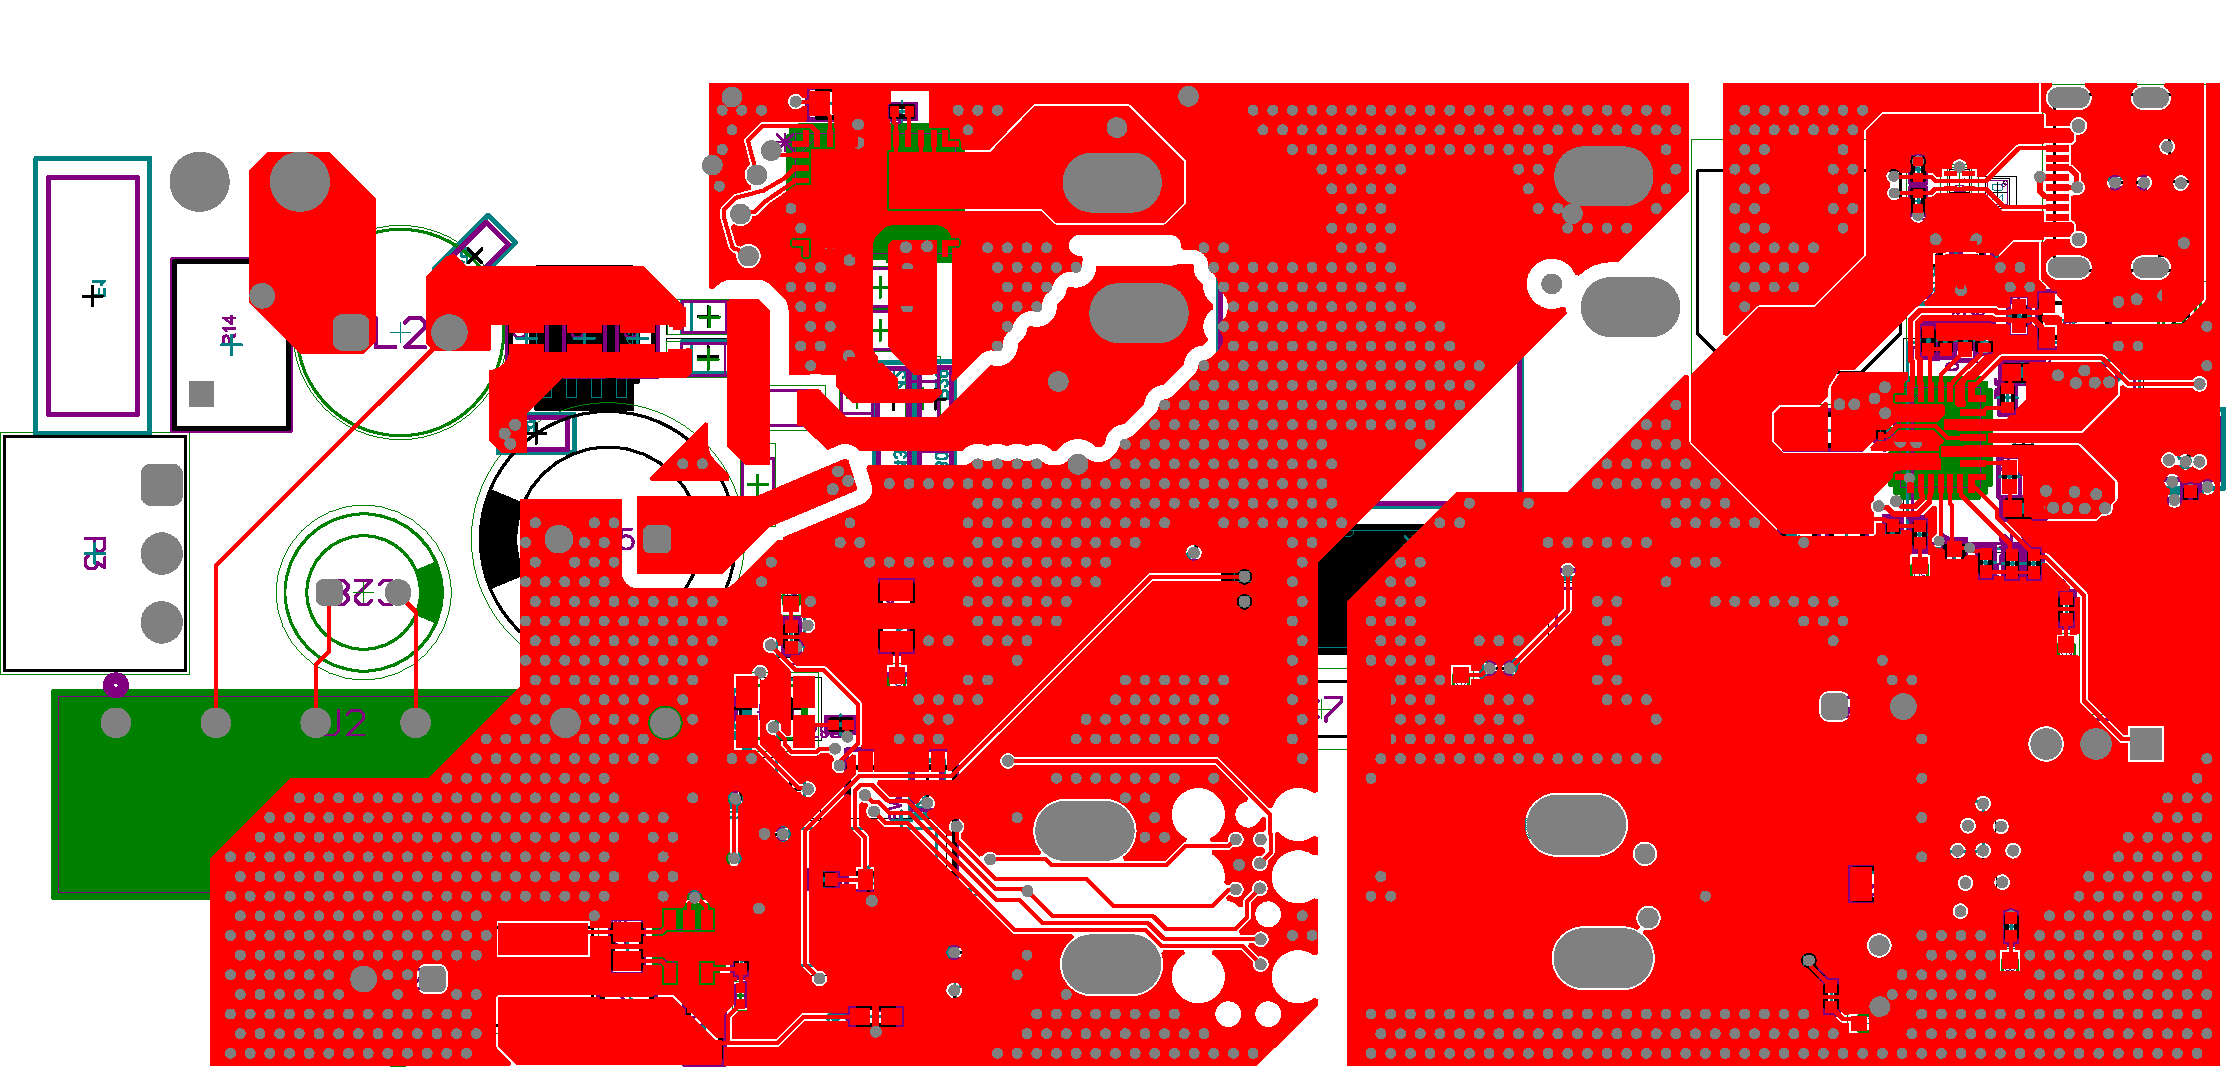
\includegraphics[page=1,width=\linewidth,height=0.33\textheight,keepaspectratio]{Pictures/Thesis/07_Hardware/PCB_V2_F410_2026-10-27.pdf}

\vspace{0.8em}
\includegraphics[page=4,width=\linewidth,height=0.33\textheight,keepaspectratio]{Pictures/Thesis/07_Hardware/PCB_V2_F410_2026-10-27.pdf}
\caption{V2 top copper (upper) and bottom copper (lower), shown in the same orientation.}
\label{fig:v2-pcb-layout-overview}
\end{figure}
\FloatBarrier

The finished board dimensions, assembly height, copper weights, and layer
thicknesses are not specified in the PCB drawings. V2 power density
therefore requires separate assembly measurements. The L4 footprint belongs
to the original resonant branch. The external inductor was removed during
the later leakage-only test described in \cref{sec:res-v2-testing}.

\subsection{Controller Connections and Timing}

The V2 carrier uses TIM1 CH1/CH1N at PA8/PB13. Moving the low-side command from PA9 and burst enable from PA10 to PA11 releases PA9/PA10 for USART1 TX/RX. Thus PA10 serves as burst enable on the G071 platform and serial receive on the F410. \Cref{tab:hw-v2-pinmap} lists the MCU pins from sheet 4 and their package pin numbers.

\begin{table}[H]
\centering
\caption{MCU pins on the G071 controller and V2 F410. Package pin numbers in the V2 column apply to the F410CBU6.}
\label{tab:hw-v2-pinmap}
\small
\begin{tabularx}{\textwidth}{@{}p{0.24\textwidth}p{0.21\textwidth}X@{}}
\toprule
Function & G071 pins & V2 F410 pins\\
\midrule
High-side carrier & PA8 & PA8, pin 29; TIM1 CH1\\
Low-side carrier & PA9 & PB13, pin 26; TIM1 CH1N\\
Power-stage enable & PA10 & PA11, pin 32; TIM5 schedules GPIO edges\\
Command UART & PC4 TX / PC5 RX & PA9 TX / PA10 RX, pins 30 / 31; J3 pins 5 / 6\\
Primary voltage & PA0 & PA0, pin 10; ADC1 channel 0\\
Secondary-bulk voltage & PA1 & PA1, pin 11; ADC1 channel 1\\
Half-bridge-current signal & PA2 & PA2, pin 12; ADC1 channel 2\\
\bottomrule
\end{tabularx}
\end{table}

The earlier V2 port configures center-aligned TIM1 at a nominal \SI{100}{\mega\hertz} timer clock, with auto-reload ARR = 50, compare CCR1 = 25, and dead-time field DTG = 4. These settings give a nominal \SI{1}{\mega\hertz} complementary carrier and \SI{40}{\nano\second} programmed dead time \cite{ststm32f410rm}. TIM5 schedules the enable envelope; bounded polling of carrier updates attempts to align non-static transitions but leaves software-dependent edge latency. The later powered trial used a reported \SI{60}{\nano\second} software setting (\cref{sec:res-v2-testing}), with its firmware version unrecorded. Effective dead time and enable alignment are measured from driver-input and switch-node captures.

ADC1 continuously scans primary voltage at PA0, secondary-bulk voltage at PA1, and half-bridge current at PA2 through DMA2 Stream0 Channel0 without synchronization to the carrier. At the \SI{25}{\mega\hertz} ADC clock, 84 acquisition and 12 conversion cycles give calculated intervals of \SI{3.84}{\micro\second} per channel and \SI{11.52}{\micro\second} per frame. Secondary-bulk voltage remains the regulated quantity; primary current supports load classification and optional protection rather than connector output-current measurement.

\subsection{Power Circuit, Sensing, and Local Supplies}

Power sheet 3 includes the LMG2652RFBR GaN half bridge, AMC0330 isolated feedback, BAC1S12SC bias supply, and two LMR54410DBVR regulators. D4, D5, D9, and D10 form the input bridge; D6--D8 form the pump diode network. All seven are labeled S4D02120T in the drawing. C25 is connected across the pumped HVVCC link, downstream of the input bridge. The primary regulator supplies \texttt{MCU\_3\_3V}; the secondary supplies \texttt{SEC\_3\_3V}. C29 is specified as \SI{1}{\micro\farad} at AUX and C30 as \SI{22}{\nano\farad} at bootstrap. The drawing also includes CAP300DG discharge, the \SI{100}{\micro\henry} L2 input inductor, three \SI{10}{\nano\farad} capacitors C21--C23, the \SI{2}{\nano\farad} C24 pump capacitor, and the \SI{10}{\micro\farad} C25 link capacitor. The parts fitted to the assembled V2 still need to be checked against the drawing.

In the resonant branch, L4 is labeled SER1512-103MED, with a nominal value of \SI{10}{\micro\henry}, but complete values or part definitions are missing for L3, T1, and C26. The external series inductor used in preliminary powered tests was reported at approximately \SI{9.4}{\micro\henry} (\cref{sec:res-v2-testing}); whether it was the component fitted at L4 has not been confirmed. The final V1.0 arrangement used two \SI{4.7}{\micro\henry} series inductors. The fitted V2 branch and transformer must be checked before calculating resonance or comparing switching waveforms.

MCU sheet 4 omits the TLV9064 buffers and connects the feedback nets directly to PA0--PA2. ADC loading and settling must therefore be checked with the actual source impedance. The code assumes a \SI{1.50}{\mega\ohm}/\SI{10}{\kilo\ohm} primary ladder, a \SI{390}{\kilo\ohm}/\SI{10}{\kilo\ohm} secondary divider, and \SI{3.3}{\volt} ADC/AMC references. R50 is labeled \SI{820}{\ohm} between the LMG2652 current-sense node and primary ground.

The divider labels do not agree with those assumptions. R29--R32 are each labeled \SI{6.2}{\mega\ohm}, and R27--R28 have the same value. Taken literally, the primary and secondary ratios are 4:1 and 2:1. These ratios do not support the intended \SI{450}{\volt} primary and \SI{28}{\volt} secondary ranges. The fitted resistor values and gain from each measured node to its ADC pin still need to be checked. Displayed voltages and voltage-protection thresholds are reliable only when the firmware conversion scales match the measured circuit.

USB-PD sheet 2 includes the MPQ4242GVE-0000-AEC1-P output stage, fed from \texttt{V\_PW\_OUTPUT\_BULK} and supplying \texttt{USB\_PD\_OUT}. The \SI{0.01}{\ohm} connector current-sense resistor is R3. This is separate from the LMG2652 sensing path on PA2. Further power-path and USB-PD tests are still needed after the preliminary powered tests in \cref{sec:res-v2-testing}.

\Needspace{0.30\textheight}
\subsection{V2 Checks and Remaining Measurements}

The October plan reports a V2 operating point near \SI{85}{\watt} and a \SI{100}{\watt} target \cite{projectOctoberPlan}. The assembly, input power, output voltage/current, temperature, duration, and firmware settings were not recorded together, so the point must be repeated with these conditions recorded. It is not included in the measured curves.

The matched \SI{79.89}{\watt} tests on the modified V1.0 assembly provide a connector-output baseline (\cref{ch:results}). Later V2 secondary-output tests reached higher power with voltage droop and continued heating (\cref{sec:res-v2-testing}); thermal-endurance tests remain incomplete. The V1.0 outline is \SI{202.77}{\milli\metre} by \SI{72.77}{\milli\metre}; V2 assembly dimensions must be measured separately before calculating its power density.
